\documentclass{beamer}


% Beamer settings
\usecolortheme{rose}
\beamertemplatenavigationsymbolsempty
\setbeamertemplate{footline}[frame number]

\titlegraphic{%

\includegraphics[height=1cm]{logo-full-colour.png}}

\addtobeamertemplate{frametitle}{}{%
\begin{tikzpicture}[remember picture,overlay]
\node[anchor=north east,yshift=2pt] at (current page.north east) {
\includegraphics[height=1cm]{logo-full-colour.png}};
\end{tikzpicture}}

% Packages
\usepackage{amsmath}

\usepackage{tikz}
\usetikzlibrary{positioning}
\usetikzlibrary{fit}

\usepackage{pgfplots}
\usepgfplotslibrary{fillbetween}

\usepackage{minted}
\usepackage[T1]{fontenc} % Required by minted to ensure dollar signs are produced instead of pound (sterling) signs

\usepackage{multicol}

\usepackage{booktabs}

\usepackage{adjustbox}

% Author
\author{Simon McIntosh-Smith \& Tom Deakin\\University of Bristol}

\date{}



\title{OpenMP for Computational Scientists}
\subtitle{5: Programming your GPU with OpenMP}

\begin{document}

\frame{\titlepage}

%-------------------------------------------------------------------------------
\begin{frame}
\frametitle{Outline}
\begin{itemize}
  \item GPU introduction
  \item The OpenMP \mintinline{fortran}|target| directive
  \item Memory movement
\end{itemize}
\end{frame}

%-------------------------------------------------------------------------------
\begin{frame}
\frametitle{GPU performance}

\begin{columns}
\begin{column}{0.5\textwidth}
\begin{adjustbox}{max width={\textwidth}}
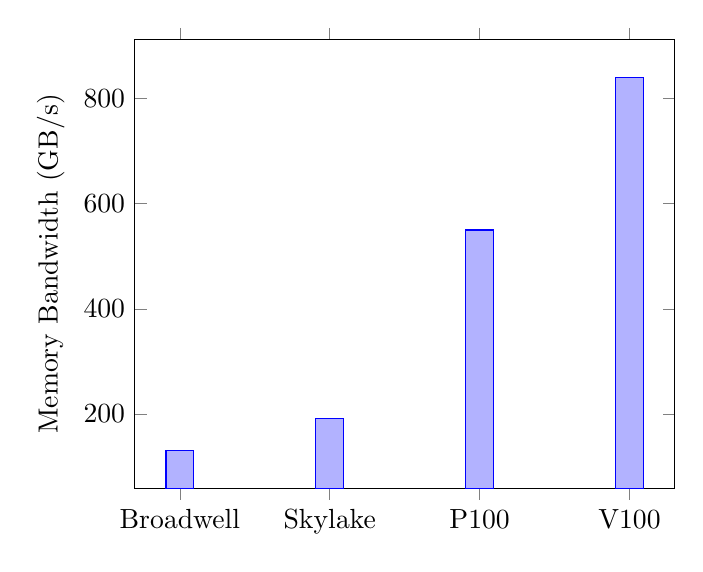
\begin{tikzpicture}
  \begin{axis}[ybar,
               symbolic x coords={Broadwell, Skylake, P100, V100},
               xtick=data,
               ylabel={Memory Bandwidth (GB/s)}]
    \addplot coordinates {(Broadwell,130) (Skylake,191) (P100,550) (V100,841)};
  \end{axis}
\end{tikzpicture}
\end{adjustbox}
\end{column}

\begin{column}{0.5\textwidth}
\begin{adjustbox}{max width={\textwidth}}
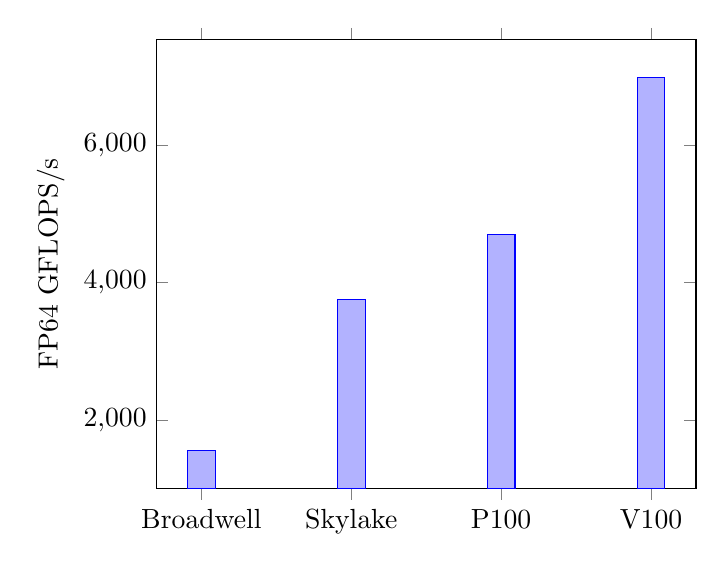
\begin{tikzpicture}
  \begin{axis}[ybar,
               symbolic x coords={Broadwell, Skylake, P100, V100},
               xtick=data,
               ylabel={FP64 GFLOPS/s}]
    \addplot coordinates {(Broadwell,1550) (Skylake,3760) (P100,4700) (V100,7000)};

  \end{axis}
\end{tikzpicture}
\end{adjustbox}
\end{column}
\end{columns}

\begin{itemize}
  \item Volta GPUs offer 4.4X memory bandwidth and 1.9X the FLOPS/s of dual-socket Skylake.
\end{itemize}

\end{frame}

%-------------------------------------------------------------------------------
\begin{frame}
\frametitle{Unlocking this potential}
\begin{itemize}
  \item GPUs made of many cores (SMs):
    \begin{itemize}
      \item V100 has 80 SMs.
      \item P100 has 56 SMs.
    \end{itemize}
  \item Each SM consists of 64 FP32 CUDA cores.
  \item CUDA cores are really organised as 2 vector units 32 wide (called warps).
\end{itemize}

\begin{block}{Take away}
GPUs are really vector-architectures made up of smaller blocks which execute together.
\end{block}
\end{frame}

%-------------------------------------------------------------------------------
\begin{frame}
\frametitle{GPUs need lots of parallelism}
\begin{itemize}
  \item GPUs are \emph{throughput optimised}, whereas CPUs are \emph{latency optimised}.
  \item Throughput optimised also called \emph{latency tolerant}.
  \item GPUs achieve this by running many operations at once, and overlapping these with each other.
  \item Hence need many (many) operations\dots
  \item A V100 has 5,120 processing elements, each needing multiple units of work to overlap.
\end{itemize}
\begin{block}{Take away}
Massive amounts of parallelism to exploit.
\end{block}
\end{frame}

%-------------------------------------------------------------------------------
\begin{frame}[fragile]
\frametitle{Device model}
\begin{itemize}
  \item OpenMP has a host/device model.
  \item Execution begins on the host CPU, with zero or more devices connected to the host.
  \item Memory spaces \emph{not} shared!
  \item Some data copied automatically, plus explicit copying.
  \item Directives are used to transfer execution to the device.
  \begin{minted}{fortran}
  !$omp target [clause [clause] ...]
  !$omp end target
  \end{minted}
  \item Host executiuon idels until target region completes (exact semantics based on tasks).
\end{itemize}

\vfill

\begin{center}
\begin{tikzpicture}
  \draw (-1,0) node {Host};
  \draw (-1,-1) node {Device};
  \draw (0,0) -- (2,0);
  \draw[dashed] (2,0) -- (3,-1);

  % GPU
  \draw (3,-1) -- (5,-1);
  \draw (3,-1.2) -- (5,-1.2);
  \draw (3,-1.4) -- (5,-1.4);
  \draw (3,-1.6) -- (5,-1.6);
  \draw (3,-0.8) -- (5,-0.8);
  \draw (3,-0.6) -- (5,-0.6);
  \draw (3,-0.4) -- (5,-0.4);

  \draw[dashed] (5,-1) -- (6,0);
  \draw[->] (6,0) -- (8,0);
\end{tikzpicture}
\end{center}
\end{frame}

%-------------------------------------------------------------------------------
\begin{frame}[fragile]
\frametitle{The target directive}
\begin{minted}{fortran}
!$omp target [clause [clause]...]
!$omp end target 
\end{minted}
\begin{itemize}
  \item Starts executing \emph{in serial} on the target device.
  \item Need other directives to expand parallelism.
  \item \mintinline{fortran}|nowait| clause:
    \begin{itemize}
      \item Allows host thread to continue working. Must synchronise later using tasks.
    \end{itemize}
  \item Other clauses mainly about memory movement, which we'll come to later.
  \item In general, you'll run loops on the device using:
  \begin{minted}[frame=single]{fortran}
  !$omp target teams distribute parallel do
  do i = 1, N
    ... ! Loop body
  end do
  !$omp end target teams distribute parallel do
  \end{minted}
\end{itemize}
\end{frame}

%-------------------------------------------------------------------------------
\begin{frame}[fragile]
\frametitle{Execution model: teams}
\begin{itemize}
  \item OpenMP \emph{threads} on a device are grouped into a \emph{team}.
  \item Can synchronise threads \emph{within} a team. \emph{Cannot} synchronise between teams.
  \item Groups of teams are called a \emph{league}.
  \item \mintinline{fortran}|target| directive offloads (serial) execution to device.
  \item \mintinline{fortran}|teams| directive creates a league of times.
  \item Master thread in each team (redundantly) executes the code.
\end{itemize}

\begin{minted}[frame=single]{fortran}
!$omp target teams 
... ! Code
!$omp end target teams
\end{minted}
\end{frame}

%-------------------------------------------------------------------------------
\begin{frame}[fragile]
\frametitle{Execution model: distribute}
\begin{itemize}
  \item Share iterations of a loop between teams.
  \item Each team gets part of the iteration space.
  \item Change default assignment with \mintinline{fortran}|dist_schedule(static)| clause. Optionally include chunk size.
  \item Still only the master thread in the team executes them.
\end{itemize}

\begin{minted}[frame=single]{fortran}
!$omp target teams distribute
do i = 1, N
... ! Code
end do
!$omp end target teams distribute
\end{minted}
\end{frame}

%-------------------------------------------------------------------------------
\begin{frame}[fragile]
\frametitle{Execution model: parallel do}
\begin{itemize}
  \item Same semantics as on the CPU!
  \item Launches threads within the team and shares iterations between threads.
  \item Note, iterations that were assigned to the team by \mintinline{fortran}|distribute| directive are shared between threads in the team.
  \item Can use the \mintinline{fortran}|schedule| clause too.
  \item Remember, can synchronise between threads in the team.
\end{itemize}

\begin{minted}[frame=single]{fortran}
!$omp target teams distribute parallel do
do i = 1, N
... ! Code
end do
!$omp end target teams distribute parallel do
\end{minted}
\end{frame}

%-------------------------------------------------------------------------------
\begin{frame}[fragile]
\frametitle{Execution example}
\begin{minted}[frame=single]{fortran}
!$omp target teams distribute parallel do
do i = 1, N
  c(i) = a(i) + b(i)
end do
!$omp end target teams distribute parallel do
\end{minted}
\end{frame}

%-------------------------------------------------------------------------------
\begin{frame}
\frametitle{Data movement}
\begin{itemize}
  \item Remember: memory is \emph{not} shared between host and target.
  \item Combination of implicit and explicit memory movement.
  \item This is the most complicated part of the offload specification.
  \item Memory movement is often a performance killer.
    \begin{itemize}
      \item A V100 has 900 GB/s peak memory bandwidth.
      \item Connected to the host via PCIe with 32 GB/s peak bandwidth.
      \item Transfers between host and device are relatively very slow: minimise them.
    \end{itemize}
\end{itemize}
\end{frame}

%-------------------------------------------------------------------------------
\begin{frame}
\frametitle{Data regions}
\begin{itemize}
  \item Data needs mapping between host and device memory spaces.
  \item Variable names exist in host and device space: the compiler sorts out which one you mean when you use them in your code.
  \item Mapping/transfers occur when
    \begin{itemize}
      \item enter/exit a \mintinline{fortran}|target| region.
      \item \mintinline{fortran}|target enter/exit data| constructs.
      \item \mintinline{fortran}|update| directives.
    \end{itemize}
  \item Default behaviour:
    \begin{itemize}
      \item Scalars are mapped \mintinline{fortran}|firstprivate|.
      \item This means the \emph{do not} get copied back to the host.
      \item Stack arrays are mapped \mintinline{fortran}|tofrom|.
      \item Heap arrays are not mapped by default.
    \end{itemize}
\end{itemize}
\end{frame}

%-------------------------------------------------------------------------------
\begin{frame}[fragile]
\frametitle{The map clause}
\begin{itemize}
  \item Specify the transfer of data between host and device on a \mintinline{fortran}|target| region.

  \item On entering the region, copy from host to device:
    \begin{minted}{fortran}
    map(to: A(1:N), x)
    \end{minted}

  \item On exiting the region, copy from device to host. At start of region, these are uninitialised on the device.
    \begin{minted}{fortran}
    map(from: A(1:N), x)
    \end{minted}

  \item Same as applying \mintinline{fortran}|map(to: ...)| and \mintinline{fortran}|map(from: ...)|
    \begin{minted}{fortran}
    map(tofrom: A(1:N), x)
    \end{minted}

  \item Allocate data on the device for use only on the device. It is uninitalised, and can't be copied back to the host.
    \begin{minted}{fortran}
    map(alloc: A(1:N))
    \end{minted}
\end{itemize}
\end{frame}

%-------------------------------------------------------------------------------
\begin{frame}[fragile]
\frametitle{Enter/exit data directives}
\begin{itemize}
  \item Often want to perform initial device data environment setup once, run through iteratative loop, copying back at end.
  \item \textbf{Do not} want to copy the data every iteration! Very expensive.
  \item Use \mintinline{fortran}|target enter data| and \mintinline{fortran}|target exit data| constructs to control device data environment.
\end{itemize}

\begin{minted}[frame=single,fontsize=\small]{fortran}
!$omp target enter data map(to: A(1:N), B(1:N), C(1:N))

do t = 1, 1000000
  !$omp target
  ... ! Read A and B, write C
  !$omp end target
end do

!$omp target exit data map(from: C(1:N))

\end{minted}
Bulk transfers happen at beginning and end, not for every \mintinline{fortran}|target| region in the big loop.
\end{frame}

%-------------------------------------------------------------------------------
\begin{frame}
\frametitle{Update directive}
\begin{itemize}
  \item Often need to transfer data between host and device between different \mintinline{fortran}|target| regions.
  \item E.g. the host does something between the two regions.
  \item Use the \mintinline{fortran}|update| directive to move the data explicitly between host and device.
  \item Example on next slide\dots
\end{itemize}
\end{frame}

%-------------------------------------------------------------------------------
\begin{frame}[fragile]
\frametitle{Update directive}
\begin{minted}[frame=single,fontsize=\small,linenos]{fortran}
!$omp target enter data map(to: A(1:N), B(1:N), C(1:N))
!$omp target
... ! Use A, B and C on device
!$omp end target

! Copy A from device to host
!$omp target update from(A(1:N))

! Change A on the host
A = 1.0

! Copy A from host to device
!$omp target update to(A(1:N))

!$omp target
... ! Use A, B and C on device
!$omp end target

!$omp target exit data map(from: C(1:N))
\end{minted}

\end{frame}

%-------------------------------------------------------------------------------
\begin{frame}[fragile]
\frametitle{Reductions}
\begin{minted}[frame=single,breaklines]{fortran}
integer :: i, N = 1000
real(kind=8), allocatable :: A(:), B(:)
real(kind=8) :: total

!$omp target map(to: A(1:N), B(1:N))
!$omp teams distribute parallel do map(tofrom:total) reduction(+:total)
do i = 1, N
  total = total + (A(i) * B(i))
end do
!$omp end teams distribute parallel do
!$omp end target
\end{minted}

\begin{itemize}
  \item \mintinline{fortran}|total| is a scalar, so by default is \mintinline{fortran}|firstprivate|.
  \item I.e. Each thread on the device gets its own copy.
  \item Importantly, it is not copied back to the host!
  \item You \emph{must} use a \mintinline{fortran}|map| clause to bring the result back.
\end{itemize}

\end{frame}

%-------------------------------------------------------------------------------
\begin{frame}
\frametitle{CUDA Toolkit: NVprof}
\begin{itemize}
  \item The CUDA toolkit works with code written in OpenMP 4.5 without any special configuration.
  \item Useful to use the profiler \mintinline{bash}|nvprof|.
  \item Particularly useful to check it ran on a GPU! Can silently fallback to CPU execution.
  \item Can generate high level profiling information, a timeline, and generate data for NVIDIA's \mintinline{bash}|nvvp| profiler.
\end{itemize}
\end{frame}

%-------------------------------------------------------------------------------
\begin{frame}[fragile]
\frametitle{nvprof output}
\begin{minted}[fontsize=\tiny]{bash}
nvprof ./stencil_target

==176642== Profiling application: ./stencil_target                                                                                                                                                                                          
==176642== Profiling result:                                                                                                                                                                                                                
Time(%)      Time     Calls       Avg       Min       Max  Name
 86.24%  424.60ms        30  14.153ms  13.776ms  14.637ms  stencil_$ck_L49_1
  9.44%  46.496ms        33  1.4090ms     895ns  24.381ms  [CUDA memcpy HtoD]
  4.31%  21.242ms        32  663.82us  1.0240us  11.176ms  [CUDA memcpy DtoH]
                                                                               
==176642== API calls:                                           
Time(%)      Time     Calls       Avg       Min       Max  Name
 53.72%  424.69ms        31  13.700ms  1.8730us  14.641ms  cuStreamSynchronize
 37.11%  293.35ms         1  293.35ms  293.35ms  293.35ms  cuCtxCreate
  5.96%  47.091ms        33  1.4270ms  6.9970us  24.584ms  cuMemcpyHtoD                 
  2.76%  21.844ms        32  682.63us  13.226us  11.304ms  cuMemcpyDtoH
  0.18%  1.4557ms         1  1.4557ms  1.4557ms  1.4557ms  cuMemHostAlloc
  0.17%  1.3477ms         5  269.54us  5.2270us  580.42us  cuMemAlloc
  0.04%  320.63us        30  10.687us  8.6930us  43.243us  cuLaunchKernel
  0.04%  317.57us         1  317.57us  317.57us  317.57us  cuModuleLoadData
  0.01%  45.755us         1  45.755us  45.755us  45.755us  cuStreamCreate
  0.00%  26.802us        34     788ns     283ns  4.3010us  cuEventCreate
  0.00%  4.3840us        11     398ns     309ns     585ns  cuDeviceGetAttribute
  0.00%  3.7440us         5     748ns     460ns  1.2540us  cuDeviceGet
  0.00%  3.6880us         3  1.2290us     356ns  2.7150us  cuDeviceGetCount
  0.00%  1.0500us         1  1.0500us  1.0500us  1.0500us  cuCtxSetCurrent
  0.00%  1.0230us         2     511ns     193ns     830ns  cuFuncGetAttribute
  0.00%     976ns         1     976ns     976ns     976ns  cuModuleGetGlobal
  0.00%     957ns         1     957ns     957ns     957ns  cuMemHostGetDevicePointer
  0.00%     806ns         1     806ns     806ns     806ns  cuModuleGetFunction
  0.00%     604ns         1     604ns     604ns     604ns  cuCtxGetCurrent
  0.00%     442ns         1     442ns     442ns     442ns  cuFuncSetCacheConfig

\end{minted}
\end{frame}

%-------------------------------------------------------------------------------
\begin{frame}[fragile]
\frametitle{nvprof output}
\begin{minted}[fontsize=\tiny,linenos,breaklines]{bash}
nvprof --print-gpu-trace ./stencil_target

==176680== Profiling application: ./stencil_target                                                                                                                                                                                  [74/200]
==176680== Profiling result:                                                                                                                                             
   Start  Duration            Grid Size      Block Size     Regs*    SSMem*    DSMem*      Size  Throughput           Device   Context    Stream  Name              
429.51ms  17.860ms                    -               -         -         -         -  122.19MB  6.6813GB/s  Tesla P100-PCIE         1         7  [CUDA memcpy HtoD]
447.94ms  15.150ms                    -               -         -         -         -  122.19MB  7.8763GB/s  Tesla P100-PCIE         1         7  [CUDA memcpy HtoD]     
463.46ms  1.4080us                    -               -         -         -         -        8B  5.4186MB/s  Tesla P100-PCIE         1         7  [CUDA memcpy HtoD]
463.47ms     992ns                    -               -         -         -         -        4B  3.8455MB/s  Tesla P100-PCIE         1         7  [CUDA memcpy HtoD]
463.90ms  14.176ms            (128 1 1)       (128 1 1)       103  1.0078KB        0B         -           -  Tesla P100-PCIE         1        14  stencil_$ck_L49_1 [43] 
478.15ms  1.5360us                    -               -         -         -         -        8B  4.9671MB/s  Tesla P100-PCIE         1         7  [CUDA memcpy DtoH]
478.61ms     992ns                    -               -         -         -         -        8B  7.6909MB/s  Tesla P100-PCIE         1         7  [CUDA memcpy HtoD]
478.63ms  14.277ms            (128 1 1)       (128 1 1)       103  1.0078KB        0B         -           -  Tesla P100-PCIE         1        14  stencil_$ck_L49_1 [79] 
492.92ms  1.1200us                    -               -         -         -         -        8B  6.8120MB/s  Tesla P100-PCIE         1         7  [CUDA memcpy DtoH]
492.96ms     992ns                    -               -         -         -         -        8B  7.6909MB/s  Tesla P100-PCIE         1         7  [CUDA memcpy HtoD]
492.97ms  14.402ms            (128 1 1)       (128 1 1)       103  1.0078KB        0B         -           -  Tesla P100-PCIE         1        14  stencil_$ck_L49_1 [83] 
507.38ms  1.3120us                    -               -         -         -         -        8B  5.8151MB/s  Tesla P100-PCIE         1         7  [CUDA memcpy DtoH]
507.41ms     992ns                    -               -         -         -         -        8B  7.6909MB/s  Tesla P100-PCIE         1         7  [CUDA memcpy HtoD]
507.43ms  14.710ms            (128 1 1)       (128 1 1)       103  1.0078KB        0B         -           -  Tesla P100-PCIE         1        14  stencil_$ck_L49_1 [87] 
522.15ms  1.3440us                    -               -         -         -         -        8B  5.6766MB/s  Tesla P100-PCIE         1         7  [CUDA memcpy DtoH]
522.18ms     992ns                    -               -         -         -         -        8B  7.6909MB/s  Tesla P100-PCIE         1         7  [CUDA memcpy HtoD]        
522.19ms  14.349ms            (128 1 1)       (128 1 1)       103  1.0078KB        0B         -           -  Tesla P100-PCIE         1        14  stencil_$ck_L49_1 [91] 
536.55ms  1.5360us                    -               -         -         -         -        8B  4.9671MB/s  Tesla P100-PCIE         1         7  [CUDA memcpy DtoH]
536.58ms     992ns                    -               -         -         -         -        8B  7.6909MB/s  Tesla P100-PCIE         1         7  [CUDA memcpy HtoD]
536.59ms  14.475ms            (128 1 1)       (128 1 1)       103  1.0078KB        0B         -           -  Tesla P100-PCIE         1        14  stencil_$ck_L49_1 [95]
551.07ms  1.1520us                    -               -         -         -         -        8B  6.6227MB/s  Tesla P100-PCIE         1         7  [CUDA memcpy DtoH]
551.10ms  1.0240us                    -               -         -         -         -        8B  7.4506MB/s  Tesla P100-PCIE         1         7  [CUDA memcpy HtoD]
551.12ms  14.233ms            (128 1 1)       (128 1 1)       103  1.0078KB        0B         -           -  Tesla P100-PCIE         1        14  stencil_$ck_L49_1 [99]
565.36ms  1.3760us                    -               -         -         -         -        8B  5.5446MB/s  Tesla P100-PCIE         1         7  [CUDA memcpy DtoH]
565.39ms     992ns                    -               -         -         -         -        8B  7.6909MB/s  Tesla P100-PCIE         1         7  [CUDA memcpy HtoD]
565.40ms  14.582ms            (128 1 1)       (128 1 1)       103  1.0078KB        0B         -           -  Tesla P100-PCIE         1        14  stencil_$ck_L49_1 [103]


\end{minted}
\end{frame}

%-------------------------------------------------------------------------------
\begin{frame}
\frametitle{Exercise}
\begin{itemize}
  \item Port your 5-point stencil code to the GPU.
  \item Use the \mintinline{fortran}|target enter/exit data| constructs to transfer data.
  \item Use the \mintinline{fortran}|target teams distribute parallel do| construct for execution.
  \item Print out the grid sum for every iteration:
    \begin{itemize}
      \item Need to use \mintinline{fortran}|reduction| clause.
      \item Remember to \mintinline{fortran}|map| the reduction result!
    \end{itemize}
  \item Extra: Think about the performance compared to your CPU version.
\end{itemize}
\end{frame}
%-------------------------------------------------------------------------------
\end{document}

